\documentclass[tikz,border=6pt]{standalone}
\usepackage{amsmath}
\usepackage{pgfplots}
\usepackage{xcolor}
\pgfplotsset{compat=1.18}

\definecolor{lineblue}{HTML}{4A90D9}
\definecolor{linegray}{HTML}{333333}

\begin{document}
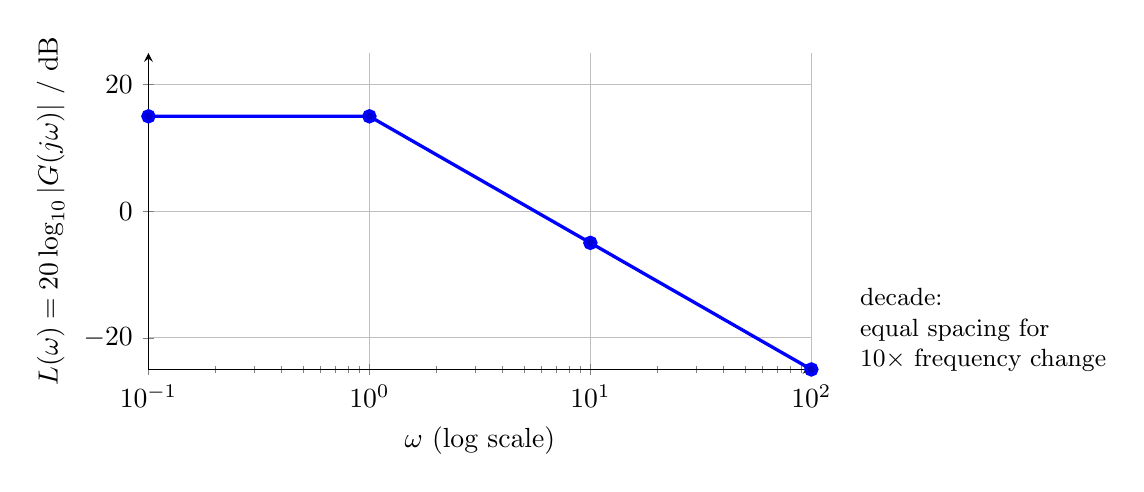
\begin{tikzpicture}
  \begin{axis}[
    width=10cm,
    height=5.6cm,
    xmode=log,
    xmin=0.1, xmax=100,
    ymin=-25, ymax=25,
    axis lines=left,
    xlabel={$\omega$ (log scale)},
    ylabel={$L(\omega)=20\log_{10}|G(j\omega)|$ / dB},
    xtick={0.1,1,10,100},
    xticklabels={$10^{-1}$,$10^0$,$10^1$,$10^2$},
    ytick={-20,0,20},
    grid=major,
    every axis plot/.append style={line width=1.2pt, color=lineblue}
  ]
    \addplot coordinates {(0.1,15) (1,15) (10,-5) (100,-25)};
  \end{axis}
  \node[align=left, font=\small] at (10.6,0.5) {decade:\\equal spacing for\\$10\times$ frequency change};
\end{tikzpicture}
\end{document}
